\section{Count ones and zeros}
\subsection{Aim}
To count the number of ones and zeroes in a given number.

\subsection{Code}
\begin{lstlisting}
ORG 0000H

MOV R0, #00H ; Resetting R0
MOV R1, #00H ; Resetting R1

MOV 10H, #0FFH ; The number
MOV R2, #08H ; Length of the number in bits

MOV A, 10H

LOOP:
	RLC A
	JC ONES
	INC R1
	JMP INC
ONES:	INC R0
INC:	DJNZ R2, LOOP

END
\end{lstlisting}

\subsection{Output}
\textbf{Input} 0F1H (R1)\\
\textbf{Output} 05 (R0) (Number of ones) and 03 (R1) number of zeros\\
\begin{center}
	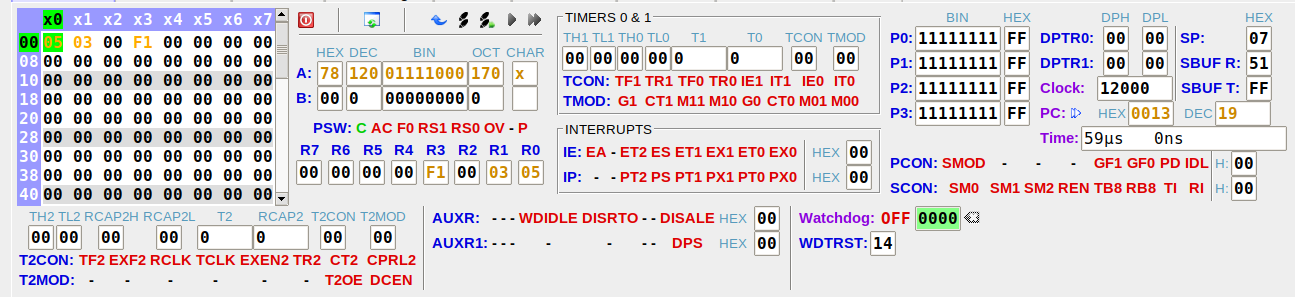
\includegraphics[width=\textwidth]{img/p25.png}
\end{center}

\subsection{Result}
The number of ones and zeros in a number was calculated in mcu8051ide